\documentclass[twoside]{book}

% Packages required by doxygen
\usepackage{fixltx2e}
\usepackage{calc}
\usepackage{doxygen}
\usepackage[export]{adjustbox} % also loads graphicx
\usepackage{graphicx}
\usepackage[utf8]{inputenc}
\usepackage{makeidx}
\usepackage{multicol}
\usepackage{multirow}
\PassOptionsToPackage{warn}{textcomp}
\usepackage{textcomp}
\usepackage[nointegrals]{wasysym}
\usepackage[table]{xcolor}

% Font selection
\usepackage[T1]{fontenc}
\usepackage[scaled=.90]{helvet}
\usepackage{courier}
\usepackage{amssymb}
\usepackage{sectsty}
\renewcommand{\familydefault}{\sfdefault}
\allsectionsfont{%
  \fontseries{bc}\selectfont%
  \color{darkgray}%
}
\renewcommand{\DoxyLabelFont}{%
  \fontseries{bc}\selectfont%
  \color{darkgray}%
}
\newcommand{\+}{\discretionary{\mbox{\scriptsize$\hookleftarrow$}}{}{}}

% Page & text layout
\usepackage{geometry}
\geometry{%
  a4paper,%
  top=2.5cm,%
  bottom=2.5cm,%
  left=2.5cm,%
  right=2.5cm%
}
\tolerance=750
\hfuzz=15pt
\hbadness=750
\setlength{\emergencystretch}{15pt}
\setlength{\parindent}{0cm}
\setlength{\parskip}{3ex plus 2ex minus 2ex}
\makeatletter
\renewcommand{\paragraph}{%
  \@startsection{paragraph}{4}{0ex}{-1.0ex}{1.0ex}{%
    \normalfont\normalsize\bfseries\SS@parafont%
  }%
}
\renewcommand{\subparagraph}{%
  \@startsection{subparagraph}{5}{0ex}{-1.0ex}{1.0ex}{%
    \normalfont\normalsize\bfseries\SS@subparafont%
  }%
}
\makeatother

% Headers & footers
\usepackage{fancyhdr}
\pagestyle{fancyplain}
\fancyhead[LE]{\fancyplain{}{\bfseries\thepage}}
\fancyhead[CE]{\fancyplain{}{}}
\fancyhead[RE]{\fancyplain{}{\bfseries\leftmark}}
\fancyhead[LO]{\fancyplain{}{\bfseries\rightmark}}
\fancyhead[CO]{\fancyplain{}{}}
\fancyhead[RO]{\fancyplain{}{\bfseries\thepage}}
\fancyfoot[LE]{\fancyplain{}{}}
\fancyfoot[CE]{\fancyplain{}{}}
\fancyfoot[RE]{\fancyplain{}{\bfseries\scriptsize Generated by Doxygen }}
\fancyfoot[LO]{\fancyplain{}{\bfseries\scriptsize Generated by Doxygen }}
\fancyfoot[CO]{\fancyplain{}{}}
\fancyfoot[RO]{\fancyplain{}{}}
\renewcommand{\footrulewidth}{0.4pt}
\renewcommand{\chaptermark}[1]{%
  \markboth{#1}{}%
}
\renewcommand{\sectionmark}[1]{%
  \markright{\thesection\ #1}%
}

% Indices & bibliography
\usepackage{natbib}
\usepackage[titles]{tocloft}
\setcounter{tocdepth}{3}
\setcounter{secnumdepth}{5}
\makeindex

% Hyperlinks (required, but should be loaded last)
\usepackage{ifpdf}
\ifpdf
  \usepackage[pdftex,pagebackref=true]{hyperref}
\else
  \usepackage[ps2pdf,pagebackref=true]{hyperref}
\fi
\hypersetup{%
  colorlinks=true,%
  linkcolor=blue,%
  citecolor=blue,%
  unicode%
}

% Custom commands
\newcommand{\clearemptydoublepage}{%
  \newpage{\pagestyle{empty}\cleardoublepage}%
}

\usepackage{caption}
\captionsetup{labelsep=space,justification=centering,font={bf},singlelinecheck=off,skip=4pt,position=top}

%===== C O N T E N T S =====

\begin{document}

% Titlepage & ToC
\hypersetup{pageanchor=false,
             bookmarksnumbered=true,
             pdfencoding=unicode
            }
\pagenumbering{alph}
\begin{titlepage}
\vspace*{7cm}
\begin{center}%
{\Large Picturasic }\\
\vspace*{1cm}
{\large Generated by Doxygen 1.8.14}\\
\end{center}
\end{titlepage}
\clearemptydoublepage
\pagenumbering{roman}
\tableofcontents
\clearemptydoublepage
\pagenumbering{arabic}
\hypersetup{pageanchor=true}

%--- Begin generated contents ---
\chapter{Hierarchical Index}
\section{Class Hierarchy}
This inheritance list is sorted roughly, but not completely, alphabetically\+:\begin{DoxyCompactList}
\item \contentsline{section}{picturazic1.\+Controlador\+Datos}{\pageref{classpicturazic1_1_1_controlador_datos}}{}
\item \contentsline{section}{picturazic1.\+D\+B\+Manager}{\pageref{classpicturazic1_1_1_d_b_manager}}{}
\item \contentsline{section}{picturazic1.\+Dynamic\+\_\+\+QR}{\pageref{classpicturazic1_1_1_dynamic___q_r}}{}
\item \contentsline{section}{modelo.\+Funciones\+Foto}{\pageref{classmodelo_1_1_funciones_foto}}{}
\item \contentsline{section}{modelo.\+Funciones\+Reto}{\pageref{classmodelo_1_1_funciones_reto}}{}
\item \contentsline{section}{modelo.\+Funciones\+Usuario}{\pageref{classmodelo_1_1_funciones_usuario}}{}
\item \contentsline{section}{picturazic1.\+Send\+Attachment\+In\+Email}{\pageref{classpicturazic1_1_1_send_attachment_in_email}}{}
\item Application\begin{DoxyCompactList}
\item \contentsline{section}{picturazic1.\+Picturazic10}{\pageref{classpicturazic1_1_1_picturazic10}}{}
\end{DoxyCompactList}
\item Initializable\begin{DoxyCompactList}
\item \contentsline{section}{picturazic1.\+Controlador\+Principal}{\pageref{classpicturazic1_1_1_controlador_principal}}{}
\item \contentsline{section}{picturazic1.\+Foto\+Controller}{\pageref{classpicturazic1_1_1_foto_controller}}{}
\item \contentsline{section}{picturazic1.\+Inicio\+Sesion\+Controller}{\pageref{classpicturazic1_1_1_inicio_sesion_controller}}{}
\item \contentsline{section}{picturazic1.\+Panel\+Comentario\+Controller}{\pageref{classpicturazic1_1_1_panel_comentario_controller}}{}
\item \contentsline{section}{picturazic1.\+Participar\+Controller}{\pageref{classpicturazic1_1_1_participar_controller}}{}
\item \contentsline{section}{picturazic1.\+Perfil\+Controller}{\pageref{classpicturazic1_1_1_perfil_controller}}{}
\item \contentsline{section}{picturazic1.\+Reto\+Controller}{\pageref{classpicturazic1_1_1_reto_controller}}{}
\end{DoxyCompactList}
\item Observable\begin{DoxyCompactList}
\item \contentsline{section}{modelo.\+Foto}{\pageref{classmodelo_1_1_foto}}{}
\item \contentsline{section}{modelo.\+Reto}{\pageref{classmodelo_1_1_reto}}{}
\item \contentsline{section}{modelo.\+Usuario}{\pageref{classmodelo_1_1_usuario}}{}
\item \contentsline{section}{picturazic1.\+Serial\+Listener}{\pageref{classpicturazic1_1_1_serial_listener}}{}
\end{DoxyCompactList}
\item Observer\begin{DoxyCompactList}
\item \contentsline{section}{picturazic1.\+Picturazic10}{\pageref{classpicturazic1_1_1_picturazic10}}{}
\end{DoxyCompactList}
\item Serial\+Port\+Event\+Listener\begin{DoxyCompactList}
\item \contentsline{section}{picturazic1.\+Picturazic10}{\pageref{classpicturazic1_1_1_picturazic10}}{}
\end{DoxyCompactList}
\end{DoxyCompactList}

\chapter{Class Index}
\section{Class List}
Here are the classes, structs, unions and interfaces with brief descriptions\+:\begin{DoxyCompactList}
\item\contentsline{section}{\mbox{\hyperlink{classpicturazic1_1_1_controlador_datos}{picturazic1.\+Controlador\+Datos}} }{\pageref{classpicturazic1_1_1_controlador_datos}}{}
\item\contentsline{section}{\mbox{\hyperlink{classpicturazic1_1_1_controlador_principal}{picturazic1.\+Controlador\+Principal}} }{\pageref{classpicturazic1_1_1_controlador_principal}}{}
\item\contentsline{section}{\mbox{\hyperlink{classpicturazic1_1_1_d_b_manager}{picturazic1.\+D\+B\+Manager}} }{\pageref{classpicturazic1_1_1_d_b_manager}}{}
\item\contentsline{section}{\mbox{\hyperlink{classpicturazic1_1_1_dynamic___q_r}{picturazic1.\+Dynamic\+\_\+\+QR}} \\*S\+A\+C\+A\+DO DE \href{http://chillyfacts.com/generate-read-qr-code-dynamically-using-java}{\tt http\+://chillyfacts.\+com/generate-\/read-\/qr-\/code-\/dynamically-\/using-\/java} }{\pageref{classpicturazic1_1_1_dynamic___q_r}}{}
\item\contentsline{section}{\mbox{\hyperlink{classmodelo_1_1_foto}{modelo.\+Foto}} }{\pageref{classmodelo_1_1_foto}}{}
\item\contentsline{section}{\mbox{\hyperlink{classpicturazic1_1_1_foto_controller}{picturazic1.\+Foto\+Controller}} }{\pageref{classpicturazic1_1_1_foto_controller}}{}
\item\contentsline{section}{\mbox{\hyperlink{classmodelo_1_1_funciones_foto}{modelo.\+Funciones\+Foto}} }{\pageref{classmodelo_1_1_funciones_foto}}{}
\item\contentsline{section}{\mbox{\hyperlink{classmodelo_1_1_funciones_reto}{modelo.\+Funciones\+Reto}} }{\pageref{classmodelo_1_1_funciones_reto}}{}
\item\contentsline{section}{\mbox{\hyperlink{classmodelo_1_1_funciones_usuario}{modelo.\+Funciones\+Usuario}} }{\pageref{classmodelo_1_1_funciones_usuario}}{}
\item\contentsline{section}{\mbox{\hyperlink{classpicturazic1_1_1_inicio_sesion_controller}{picturazic1.\+Inicio\+Sesion\+Controller}} }{\pageref{classpicturazic1_1_1_inicio_sesion_controller}}{}
\item\contentsline{section}{\mbox{\hyperlink{classpicturazic1_1_1_panel_comentario_controller}{picturazic1.\+Panel\+Comentario\+Controller}} }{\pageref{classpicturazic1_1_1_panel_comentario_controller}}{}
\item\contentsline{section}{\mbox{\hyperlink{classpicturazic1_1_1_participar_controller}{picturazic1.\+Participar\+Controller}} }{\pageref{classpicturazic1_1_1_participar_controller}}{}
\item\contentsline{section}{\mbox{\hyperlink{classpicturazic1_1_1_perfil_controller}{picturazic1.\+Perfil\+Controller}} }{\pageref{classpicturazic1_1_1_perfil_controller}}{}
\item\contentsline{section}{\mbox{\hyperlink{classpicturazic1_1_1_picturazic10}{picturazic1.\+Picturazic10}} }{\pageref{classpicturazic1_1_1_picturazic10}}{}
\item\contentsline{section}{\mbox{\hyperlink{classmodelo_1_1_reto}{modelo.\+Reto}} }{\pageref{classmodelo_1_1_reto}}{}
\item\contentsline{section}{\mbox{\hyperlink{classpicturazic1_1_1_reto_controller}{picturazic1.\+Reto\+Controller}} }{\pageref{classpicturazic1_1_1_reto_controller}}{}
\item\contentsline{section}{\mbox{\hyperlink{classpicturazic1_1_1_send_attachment_in_email}{picturazic1.\+Send\+Attachment\+In\+Email}} }{\pageref{classpicturazic1_1_1_send_attachment_in_email}}{}
\item\contentsline{section}{\mbox{\hyperlink{classpicturazic1_1_1_serial_listener}{picturazic1.\+Serial\+Listener}} }{\pageref{classpicturazic1_1_1_serial_listener}}{}
\item\contentsline{section}{\mbox{\hyperlink{classmodelo_1_1_usuario}{modelo.\+Usuario}} }{\pageref{classmodelo_1_1_usuario}}{}
\end{DoxyCompactList}

\chapter{Class Documentation}
\hypertarget{classpicturazic1_1_1_controlador_datos}{}\section{picturazic1.\+Controlador\+Datos Class Reference}
\label{classpicturazic1_1_1_controlador_datos}\index{picturazic1.\+Controlador\+Datos@{picturazic1.\+Controlador\+Datos}}
\subsection*{Public Member Functions}
\begin{DoxyCompactItemize}
\item 
\mbox{\Hypertarget{classpicturazic1_1_1_controlador_datos_a82815ab2c79255c6087dbc0165d917bd}\label{classpicturazic1_1_1_controlador_datos_a82815ab2c79255c6087dbc0165d917bd}} 
boolean {\bfseries crear\+Conecxion} ()  throws S\+Q\+L\+Exception 
\item 
\mbox{\Hypertarget{classpicturazic1_1_1_controlador_datos_ac929336070f713ca3cdc703b1a76a070}\label{classpicturazic1_1_1_controlador_datos_ac929336070f713ca3cdc703b1a76a070}} 
void {\bfseries inicializar\+Usuario} ()
\item 
\mbox{\Hypertarget{classpicturazic1_1_1_controlador_datos_a44a859236ba011fa557e718379f50018}\label{classpicturazic1_1_1_controlador_datos_a44a859236ba011fa557e718379f50018}} 
\mbox{\hyperlink{classmodelo_1_1_usuario}{Usuario}} {\bfseries obtener\+Usuario} ()
\end{DoxyCompactItemize}


\subsection{Detailed Description}
\begin{DoxyAuthor}{Author}
HW 
\end{DoxyAuthor}


The documentation for this class was generated from the following file\+:\begin{DoxyCompactItemize}
\item 
D\+:/\+Escritorio/\+Clase/20172018/\+Eclipse Workspace/\+Picturasic/src/picturazic1/Controlador\+Datos.\+java\end{DoxyCompactItemize}

\hypertarget{classpicturazic1_1_1_controlador_principal}{}\section{picturazic1.\+Controlador\+Principal Class Reference}
\label{classpicturazic1_1_1_controlador_principal}\index{picturazic1.\+Controlador\+Principal@{picturazic1.\+Controlador\+Principal}}
Inheritance diagram for picturazic1.\+Controlador\+Principal\+:\begin{figure}[H]
\begin{center}
\leavevmode
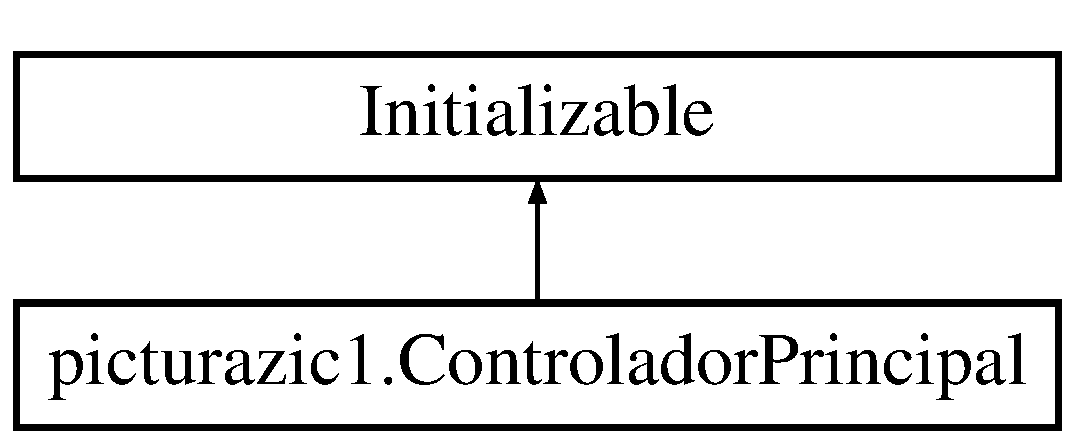
\includegraphics[height=2.000000cm]{classpicturazic1_1_1_controlador_principal}
\end{center}
\end{figure}
\subsection*{Public Member Functions}
\begin{DoxyCompactItemize}
\item 
void \mbox{\hyperlink{classpicturazic1_1_1_controlador_principal_aceb559cae1605639bcf18d28c48fa738}{initialize}} (U\+RL url, Resource\+Bundle rb)
\item 
\mbox{\Hypertarget{classpicturazic1_1_1_controlador_principal_a0f901b475d9d579f91b6553ff24f7989}\label{classpicturazic1_1_1_controlador_principal_a0f901b475d9d579f91b6553ff24f7989}} 
void {\bfseries obtener\+Stage} (Stage s, \mbox{\hyperlink{classmodelo_1_1_usuario}{Usuario}} u, \mbox{\hyperlink{classpicturazic1_1_1_picturazic10}{Picturazic10}} ob)
\item 
\mbox{\Hypertarget{classpicturazic1_1_1_controlador_principal_a25a24ea8169d64e2521ba7fbe0ad3be4}\label{classpicturazic1_1_1_controlador_principal_a25a24ea8169d64e2521ba7fbe0ad3be4}} 
void {\bfseries inicializar\+Usuario} (\mbox{\hyperlink{classmodelo_1_1_usuario}{Usuario}} usuario)
\item 
\mbox{\Hypertarget{classpicturazic1_1_1_controlador_principal_a96871e61884a5b0ad647b9637d60eb0f}\label{classpicturazic1_1_1_controlador_principal_a96871e61884a5b0ad647b9637d60eb0f}} 
void {\bfseries cargar\+Perfil} (int id, \mbox{\hyperlink{classmodelo_1_1_usuario}{Usuario}} u)  throws I\+O\+Exception 
\item 
\mbox{\Hypertarget{classpicturazic1_1_1_controlador_principal_a51c6c72cac7befd2d89ba1d7c15afc25}\label{classpicturazic1_1_1_controlador_principal_a51c6c72cac7befd2d89ba1d7c15afc25}} 
void {\bfseries participar\+Reto} (\mbox{\hyperlink{classmodelo_1_1_reto}{Reto}} o)  throws I\+O\+Exception 
\item 
\mbox{\Hypertarget{classpicturazic1_1_1_controlador_principal_ae8ce2539007dd9d05f9d766c7818bfb1}\label{classpicturazic1_1_1_controlador_principal_ae8ce2539007dd9d05f9d766c7818bfb1}} 
void {\bfseries visualizar\+Fotos} (List$<$ \mbox{\hyperlink{classmodelo_1_1_foto}{Foto}} $>$ lista)  throws I\+O\+Exception 
\item 
\mbox{\Hypertarget{classpicturazic1_1_1_controlador_principal_ac62cbb41a2404c86d838c399a8d00ee7}\label{classpicturazic1_1_1_controlador_principal_ac62cbb41a2404c86d838c399a8d00ee7}} 
void {\bfseries visualizar\+Fotos\+Usuario} (List$<$ \mbox{\hyperlink{classmodelo_1_1_foto}{Foto}} $>$ lista)  throws I\+O\+Exception 
\item 
\mbox{\Hypertarget{classpicturazic1_1_1_controlador_principal_a40b14259c066a2db168f6f2e7392b63b}\label{classpicturazic1_1_1_controlador_principal_a40b14259c066a2db168f6f2e7392b63b}} 
void {\bfseries visualizar\+Usuarios} (List$<$ \mbox{\hyperlink{classmodelo_1_1_usuario}{Usuario}} $>$ lista)  throws I\+O\+Exception 
\item 
\mbox{\Hypertarget{classpicturazic1_1_1_controlador_principal_a3be9dac836f03754f365e4b221b540e3}\label{classpicturazic1_1_1_controlador_principal_a3be9dac836f03754f365e4b221b540e3}} 
void {\bfseries visualizar\+Retos} (List$<$ \mbox{\hyperlink{classmodelo_1_1_reto}{Reto}} $>$ lista, \mbox{\hyperlink{classpicturazic1_1_1_picturazic10}{Picturazic10}} obse)  throws I\+O\+Exception 
\end{DoxyCompactItemize}


\subsection{Detailed Description}
F\+X\+ML Controller class

\begin{DoxyAuthor}{Author}
HW 
\end{DoxyAuthor}


\subsection{Member Function Documentation}
\mbox{\Hypertarget{classpicturazic1_1_1_controlador_principal_aceb559cae1605639bcf18d28c48fa738}\label{classpicturazic1_1_1_controlador_principal_aceb559cae1605639bcf18d28c48fa738}} 
\index{picturazic1\+::\+Controlador\+Principal@{picturazic1\+::\+Controlador\+Principal}!initialize@{initialize}}
\index{initialize@{initialize}!picturazic1\+::\+Controlador\+Principal@{picturazic1\+::\+Controlador\+Principal}}
\subsubsection{\texorpdfstring{initialize()}{initialize()}}
{\footnotesize\ttfamily void picturazic1.\+Controlador\+Principal.\+initialize (\begin{DoxyParamCaption}\item[{U\+RL}]{url,  }\item[{Resource\+Bundle}]{rb }\end{DoxyParamCaption})}

Initializes the controller class. 

The documentation for this class was generated from the following file\+:\begin{DoxyCompactItemize}
\item 
D\+:/\+Escritorio/\+Clase/20172018/\+Eclipse Workspace/\+Picturasic/src/picturazic1/Controlador\+Principal.\+java\end{DoxyCompactItemize}

\hypertarget{classpicturazic1_1_1_d_b_manager}{}\section{picturazic1.\+D\+B\+Manager Class Reference}
\label{classpicturazic1_1_1_d_b_manager}\index{picturazic1.\+D\+B\+Manager@{picturazic1.\+D\+B\+Manager}}
\subsection*{Static Public Member Functions}
\begin{DoxyCompactItemize}
\item 
\mbox{\Hypertarget{classpicturazic1_1_1_d_b_manager_a8f88c3dfad4434f6704a272bfb031fa6}\label{classpicturazic1_1_1_d_b_manager_a8f88c3dfad4434f6704a272bfb031fa6}} 
static Connection {\bfseries get\+Connection} ()
\end{DoxyCompactItemize}


\subsection{Detailed Description}
\begin{DoxyAuthor}{Author}
HW 
\end{DoxyAuthor}


The documentation for this class was generated from the following file\+:\begin{DoxyCompactItemize}
\item 
D\+:/\+Escritorio/\+Clase/20172018/\+Eclipse Workspace/\+Picturasic/src/picturazic1/D\+B\+Manager.\+java\end{DoxyCompactItemize}

\hypertarget{classpicturazic1_1_1_dynamic___q_r}{}\section{picturazic1.\+Dynamic\+\_\+\+QR Class Reference}
\label{classpicturazic1_1_1_dynamic___q_r}\index{picturazic1.\+Dynamic\+\_\+\+QR@{picturazic1.\+Dynamic\+\_\+\+QR}}


S\+A\+C\+A\+DO DE \href{http://chillyfacts.com/generate-read-qr-code-dynamically-using-java}{\tt http\+://chillyfacts.\+com/generate-\/read-\/qr-\/code-\/dynamically-\/using-\/java}.  


\subsection*{Static Public Member Functions}
\begin{DoxyCompactItemize}
\item 
\mbox{\Hypertarget{classpicturazic1_1_1_dynamic___q_r_aac67582f2765a22cd14e8d7470ca699f}\label{classpicturazic1_1_1_dynamic___q_r_aac67582f2765a22cd14e8d7470ca699f}} 
static String {\bfseries encriptar} (String txt)
\item 
\mbox{\Hypertarget{classpicturazic1_1_1_dynamic___q_r_af19cbcbd1b21b2a863289c51a600546a}\label{classpicturazic1_1_1_dynamic___q_r_af19cbcbd1b21b2a863289c51a600546a}} 
static void {\bfseries generate\+\_\+qr} (String image\+\_\+name, String str, String email)
\end{DoxyCompactItemize}


\subsection{Detailed Description}
S\+A\+C\+A\+DO DE \href{http://chillyfacts.com/generate-read-qr-code-dynamically-using-java}{\tt http\+://chillyfacts.\+com/generate-\/read-\/qr-\/code-\/dynamically-\/using-\/java}. 

The documentation for this class was generated from the following file\+:\begin{DoxyCompactItemize}
\item 
D\+:/\+Escritorio/\+Clase/20172018/\+Eclipse Workspace/\+Picturasic/src/picturazic1/Dynamic\+\_\+\+Q\+R.\+java\end{DoxyCompactItemize}

\hypertarget{classmodelo_1_1_foto}{}\section{modelo.\+Foto Class Reference}
\label{classmodelo_1_1_foto}\index{modelo.\+Foto@{modelo.\+Foto}}
Inheritance diagram for modelo.\+Foto\+:\begin{figure}[H]
\begin{center}
\leavevmode
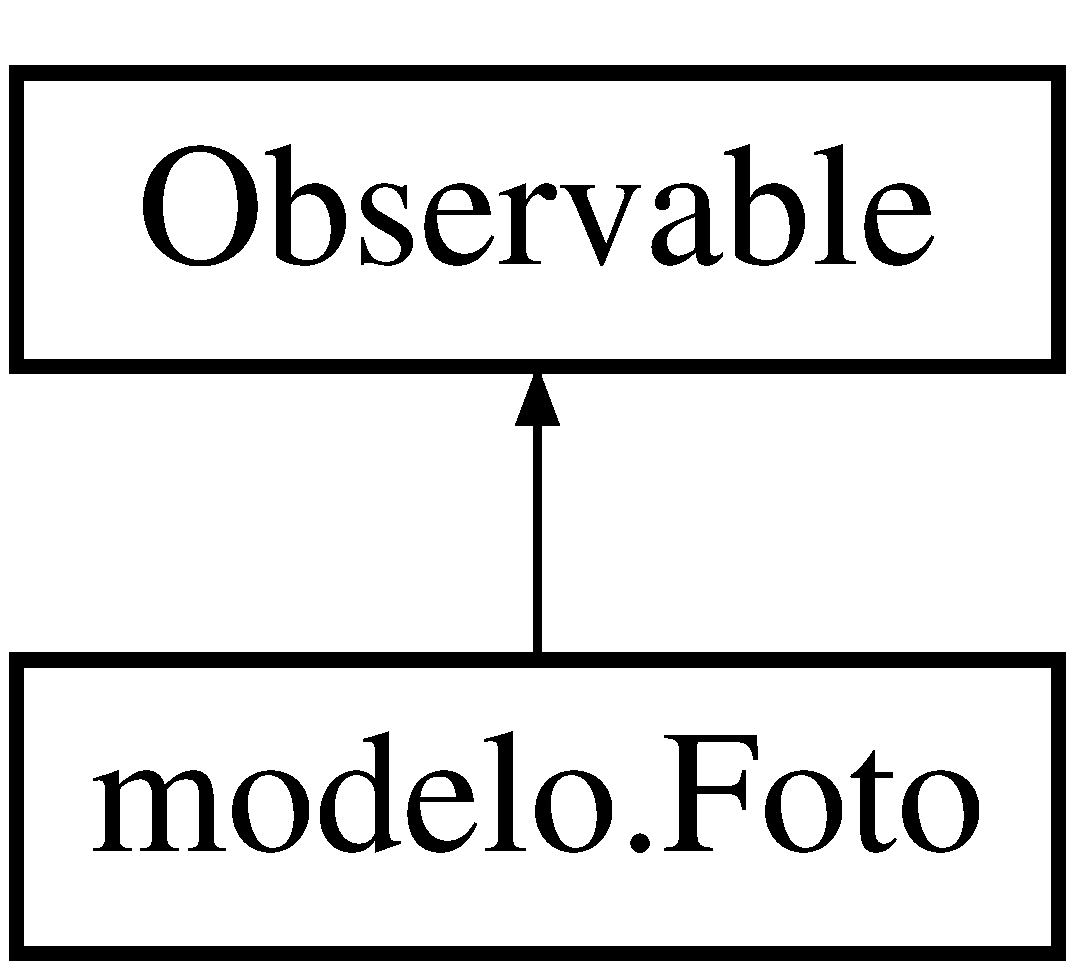
\includegraphics[height=2.000000cm]{classmodelo_1_1_foto}
\end{center}
\end{figure}
\subsection*{Public Member Functions}
\begin{DoxyCompactItemize}
\item 
\mbox{\Hypertarget{classmodelo_1_1_foto_a4ae8adb7dd9fd3cec9a8773232f66a1d}\label{classmodelo_1_1_foto_a4ae8adb7dd9fd3cec9a8773232f66a1d}} 
{\bfseries Foto} (int id, int reto\+Id, Buffered\+Image imagen, int usuario\+Id)
\item 
\mbox{\Hypertarget{classmodelo_1_1_foto_a9b0059a5f5b4dfddd3361da5479c4fae}\label{classmodelo_1_1_foto_a9b0059a5f5b4dfddd3361da5479c4fae}} 
void {\bfseries ver\+Comentarios} ()
\item 
\mbox{\Hypertarget{classmodelo_1_1_foto_a829de9aa94b0955e74c40d227e5c301a}\label{classmodelo_1_1_foto_a829de9aa94b0955e74c40d227e5c301a}} 
void {\bfseries megusta} (int usuario)  throws S\+Q\+L\+Exception 
\item 
\mbox{\Hypertarget{classmodelo_1_1_foto_a35904c75dd74f11b2551af25ab3e98d1}\label{classmodelo_1_1_foto_a35904c75dd74f11b2551af25ab3e98d1}} 
void {\bfseries borrar\+Foto} ()
\item 
\mbox{\Hypertarget{classmodelo_1_1_foto_ae92de210d35310e441ac83f66f856017}\label{classmodelo_1_1_foto_ae92de210d35310e441ac83f66f856017}} 
int {\bfseries get\+Id} ()
\item 
\mbox{\Hypertarget{classmodelo_1_1_foto_a499b7f4c02e897250fd5706a5f54faa8}\label{classmodelo_1_1_foto_a499b7f4c02e897250fd5706a5f54faa8}} 
int {\bfseries get\+Reto\+Id} ()
\item 
\mbox{\Hypertarget{classmodelo_1_1_foto_a1c1a774410b574bd94023b050089277d}\label{classmodelo_1_1_foto_a1c1a774410b574bd94023b050089277d}} 
Buffered\+Image {\bfseries get\+Imagen} ()
\item 
\mbox{\Hypertarget{classmodelo_1_1_foto_a5233c028ac855ccf38d0de3c97c64152}\label{classmodelo_1_1_foto_a5233c028ac855ccf38d0de3c97c64152}} 
int {\bfseries get\+Usuario\+Id} ()
\item 
\mbox{\Hypertarget{classmodelo_1_1_foto_a53afa33e0df03c6ed782a2cfe6d52112}\label{classmodelo_1_1_foto_a53afa33e0df03c6ed782a2cfe6d52112}} 
String {\bfseries obtener\+Likes} ()
\end{DoxyCompactItemize}
\subsection*{Static Public Member Functions}
\begin{DoxyCompactItemize}
\item 
\mbox{\Hypertarget{classmodelo_1_1_foto_adcf36212769d687253077abfe7ec718d}\label{classmodelo_1_1_foto_adcf36212769d687253077abfe7ec718d}} 
static List$<$ \mbox{\hyperlink{classmodelo_1_1_foto}{Foto}} $>$ {\bfseries obtener\+Fotos\+Usuario} (int id)
\item 
\mbox{\Hypertarget{classmodelo_1_1_foto_a09d5bb0737c55dc05004cf7e1c9d6095}\label{classmodelo_1_1_foto_a09d5bb0737c55dc05004cf7e1c9d6095}} 
static List$<$ \mbox{\hyperlink{classmodelo_1_1_foto}{Foto}} $>$ {\bfseries obtener\+Fotos\+Populares} ()
\item 
\mbox{\Hypertarget{classmodelo_1_1_foto_a6d2db8c4412bb95eb8c4b7c9e5849608}\label{classmodelo_1_1_foto_a6d2db8c4412bb95eb8c4b7c9e5849608}} 
static List$<$ \mbox{\hyperlink{classmodelo_1_1_foto}{Foto}} $>$ {\bfseries obtener\+Foto\+Seguidos} (int id)
\end{DoxyCompactItemize}


\subsection{Detailed Description}
\begin{DoxyAuthor}{Author}
HW 
\end{DoxyAuthor}


The documentation for this class was generated from the following file\+:\begin{DoxyCompactItemize}
\item 
D\+:/\+Escritorio/\+Clase/20172018/\+Eclipse Workspace/\+Picturasic/src/modelo/Foto.\+java\end{DoxyCompactItemize}

\hypertarget{classpicturazic1_1_1_foto_controller}{}\section{picturazic1.\+Foto\+Controller Class Reference}
\label{classpicturazic1_1_1_foto_controller}\index{picturazic1.\+Foto\+Controller@{picturazic1.\+Foto\+Controller}}
Inheritance diagram for picturazic1.\+Foto\+Controller\+:\begin{figure}[H]
\begin{center}
\leavevmode
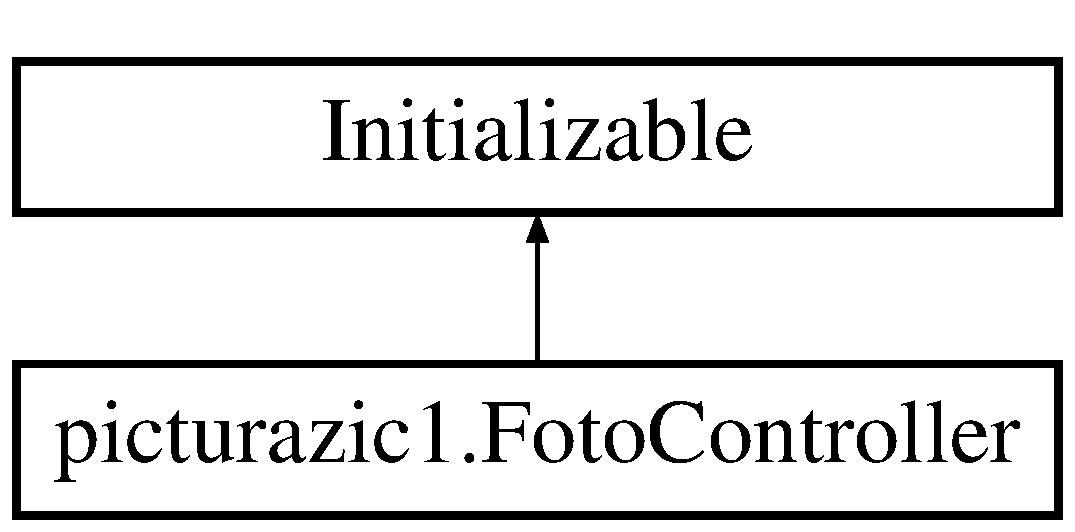
\includegraphics[height=2.000000cm]{classpicturazic1_1_1_foto_controller}
\end{center}
\end{figure}
\subsection*{Public Member Functions}
\begin{DoxyCompactItemize}
\item 
void \mbox{\hyperlink{classpicturazic1_1_1_foto_controller_a3703f1afb84525455d11c18c49dc0499}{initialize}} (U\+RL url, Resource\+Bundle rb)
\item 
\mbox{\Hypertarget{classpicturazic1_1_1_foto_controller_a05c242e320f8c6e4221b9ed027afc355}\label{classpicturazic1_1_1_foto_controller_a05c242e320f8c6e4221b9ed027afc355}} 
void {\bfseries crear\+Foto} (\mbox{\hyperlink{classmodelo_1_1_foto}{Foto}} foto, \mbox{\hyperlink{classmodelo_1_1_usuario}{Usuario}} u, \mbox{\hyperlink{classpicturazic1_1_1_picturazic10}{Picturazic10}} a)
\end{DoxyCompactItemize}


\subsection{Detailed Description}
F\+X\+ML Controller class

\begin{DoxyAuthor}{Author}
HW 
\end{DoxyAuthor}


\subsection{Member Function Documentation}
\mbox{\Hypertarget{classpicturazic1_1_1_foto_controller_a3703f1afb84525455d11c18c49dc0499}\label{classpicturazic1_1_1_foto_controller_a3703f1afb84525455d11c18c49dc0499}} 
\index{picturazic1\+::\+Foto\+Controller@{picturazic1\+::\+Foto\+Controller}!initialize@{initialize}}
\index{initialize@{initialize}!picturazic1\+::\+Foto\+Controller@{picturazic1\+::\+Foto\+Controller}}
\subsubsection{\texorpdfstring{initialize()}{initialize()}}
{\footnotesize\ttfamily void picturazic1.\+Foto\+Controller.\+initialize (\begin{DoxyParamCaption}\item[{U\+RL}]{url,  }\item[{Resource\+Bundle}]{rb }\end{DoxyParamCaption})}

Initializes the controller class. 

The documentation for this class was generated from the following file\+:\begin{DoxyCompactItemize}
\item 
D\+:/\+Escritorio/\+Clase/20172018/\+Eclipse Workspace/\+Picturasic/src/picturazic1/Foto\+Controller.\+java\end{DoxyCompactItemize}

\hypertarget{classmodelo_1_1_funciones_foto}{}\section{modelo.\+Funciones\+Foto Class Reference}
\label{classmodelo_1_1_funciones_foto}\index{modelo.\+Funciones\+Foto@{modelo.\+Funciones\+Foto}}
\subsection*{Static Public Member Functions}
\begin{DoxyCompactItemize}
\item 
\mbox{\Hypertarget{classmodelo_1_1_funciones_foto_a2006de20388ea2c3daec2fd76d3fdd6c}\label{classmodelo_1_1_funciones_foto_a2006de20388ea2c3daec2fd76d3fdd6c}} 
static List$<$ \mbox{\hyperlink{classmodelo_1_1_foto}{Foto}} $>$ {\bfseries get\+Fotos\+Usuario} (int id\+Usuario)
\item 
\mbox{\Hypertarget{classmodelo_1_1_funciones_foto_a883115b8c978380b7449944ff0084b9e}\label{classmodelo_1_1_funciones_foto_a883115b8c978380b7449944ff0084b9e}} 
static List$<$ \mbox{\hyperlink{classmodelo_1_1_foto}{Foto}} $>$ {\bfseries get\+Fotos\+Seguidos} (int id\+Usuario)
\item 
\mbox{\Hypertarget{classmodelo_1_1_funciones_foto_a3d8bd570b4ca297805600c4156d47e62}\label{classmodelo_1_1_funciones_foto_a3d8bd570b4ca297805600c4156d47e62}} 
static String {\bfseries get\+Likes} (int fotoid)
\item 
\mbox{\Hypertarget{classmodelo_1_1_funciones_foto_afafc5c872db03a4f492b1978737b723e}\label{classmodelo_1_1_funciones_foto_afafc5c872db03a4f492b1978737b723e}} 
static void {\bfseries anadir\+Foto} (String descripcion, int autor\+Id, int reto\+Id, String img\+Path, String fecha)
\item 
\mbox{\Hypertarget{classmodelo_1_1_funciones_foto_a1e5c2c4f44a64457c5d110c7cef49177}\label{classmodelo_1_1_funciones_foto_a1e5c2c4f44a64457c5d110c7cef49177}} 
static void {\bfseries anadir\+Megusta} (int foto\+Id, int usuario)  throws S\+Q\+L\+Exception 
\end{DoxyCompactItemize}


\subsection{Detailed Description}
\begin{DoxyAuthor}{Author}
HW 
\end{DoxyAuthor}


The documentation for this class was generated from the following file\+:\begin{DoxyCompactItemize}
\item 
D\+:/\+Escritorio/\+Clase/20172018/\+Eclipse Workspace/\+Picturasic/src/modelo/Funciones\+Foto.\+java\end{DoxyCompactItemize}

\hypertarget{classmodelo_1_1_funciones_reto}{}\section{modelo.\+Funciones\+Reto Class Reference}
\label{classmodelo_1_1_funciones_reto}\index{modelo.\+Funciones\+Reto@{modelo.\+Funciones\+Reto}}
\subsection*{Static Public Member Functions}
\begin{DoxyCompactItemize}
\item 
\mbox{\Hypertarget{classmodelo_1_1_funciones_reto_acd04f7cb0f62cd2e1d36922b2c5584c1}\label{classmodelo_1_1_funciones_reto_acd04f7cb0f62cd2e1d36922b2c5584c1}} 
static void {\bfseries anadir\+Reto} (String descripcion, String img\+Path)
\item 
\mbox{\Hypertarget{classmodelo_1_1_funciones_reto_aaf96317180eb9b0ae75e5873892d737a}\label{classmodelo_1_1_funciones_reto_aaf96317180eb9b0ae75e5873892d737a}} 
static void {\bfseries actualizar\+Foto\+Reto} (int id\+Reto, String img\+Path)
\item 
\mbox{\Hypertarget{classmodelo_1_1_funciones_reto_a255822dd6c53518e851e9f947772538c}\label{classmodelo_1_1_funciones_reto_a255822dd6c53518e851e9f947772538c}} 
static List$<$ \mbox{\hyperlink{classmodelo_1_1_reto}{Reto}} $>$ {\bfseries buscar\+Reto} (int id\+User)
\end{DoxyCompactItemize}


\subsection{Detailed Description}
\begin{DoxyAuthor}{Author}
HW 
\end{DoxyAuthor}


The documentation for this class was generated from the following file\+:\begin{DoxyCompactItemize}
\item 
D\+:/\+Escritorio/\+Clase/20172018/\+Eclipse Workspace/\+Picturasic/src/modelo/Funciones\+Reto.\+java\end{DoxyCompactItemize}

\hypertarget{classmodelo_1_1_funciones_usuario}{}\section{modelo.\+Funciones\+Usuario Class Reference}
\label{classmodelo_1_1_funciones_usuario}\index{modelo.\+Funciones\+Usuario@{modelo.\+Funciones\+Usuario}}
\subsection*{Static Public Member Functions}
\begin{DoxyCompactItemize}
\item 
\mbox{\Hypertarget{classmodelo_1_1_funciones_usuario_a49d730e1fcebc465cf791fce48a34b95}\label{classmodelo_1_1_funciones_usuario_a49d730e1fcebc465cf791fce48a34b95}} 
static List$<$ \mbox{\hyperlink{classmodelo_1_1_usuario}{Usuario}} $>$ {\bfseries buscar\+Usuario} (String busqueda, int id)
\item 
\mbox{\Hypertarget{classmodelo_1_1_funciones_usuario_a6325b50dfce4ac36643c5ebbb03e931e}\label{classmodelo_1_1_funciones_usuario_a6325b50dfce4ac36643c5ebbb03e931e}} 
static List$<$ \mbox{\hyperlink{classmodelo_1_1_usuario}{Usuario}} $>$ {\bfseries buscar\+Seguidores} (int id)
\item 
\mbox{\Hypertarget{classmodelo_1_1_funciones_usuario_a7cdfd051909a2d4dccc72b036980a361}\label{classmodelo_1_1_funciones_usuario_a7cdfd051909a2d4dccc72b036980a361}} 
static void {\bfseries sguir} (int seguidor, int seguido)  throws S\+Q\+L\+Exception 
\item 
\mbox{\Hypertarget{classmodelo_1_1_funciones_usuario_a9da64b56e0ac7478737d48d4260fe745}\label{classmodelo_1_1_funciones_usuario_a9da64b56e0ac7478737d48d4260fe745}} 
static void {\bfseries anadir\+Usuario} (String usuario, String correo, String nombre, String apellido, boolean admin, String pass)
\item 
\mbox{\Hypertarget{classmodelo_1_1_funciones_usuario_acd3a29fd9df1482fba1fdd6628d7d6ee}\label{classmodelo_1_1_funciones_usuario_acd3a29fd9df1482fba1fdd6628d7d6ee}} 
static void {\bfseries actualizar\+Avatar} (String img\+Path, int id\+Usuario)
\item 
\mbox{\Hypertarget{classmodelo_1_1_funciones_usuario_a7b1637ae715ceea91d9884026ead80b6}\label{classmodelo_1_1_funciones_usuario_a7b1637ae715ceea91d9884026ead80b6}} 
static Buffered\+Image {\bfseries get\+Avatar} (int id\+Usuario)
\item 
\mbox{\Hypertarget{classmodelo_1_1_funciones_usuario_a054d140d4835b763885af853ce4065d5}\label{classmodelo_1_1_funciones_usuario_a054d140d4835b763885af853ce4065d5}} 
static void {\bfseries sumar\+Exp} (int id\+Usuario, int exp\+Sumar)
\item 
\mbox{\Hypertarget{classmodelo_1_1_funciones_usuario_ae21c08bf2452095f1b71e6b5e1ef56a7}\label{classmodelo_1_1_funciones_usuario_ae21c08bf2452095f1b71e6b5e1ef56a7}} 
static \mbox{\hyperlink{classmodelo_1_1_usuario}{Usuario}} {\bfseries buscar\+Usuario\+Por\+Id} (int id)
\end{DoxyCompactItemize}


\subsection{Detailed Description}
\begin{DoxyAuthor}{Author}
HW 
\end{DoxyAuthor}


The documentation for this class was generated from the following file\+:\begin{DoxyCompactItemize}
\item 
D\+:/\+Escritorio/\+Clase/20172018/\+Eclipse Workspace/\+Picturasic/src/modelo/Funciones\+Usuario.\+java\end{DoxyCompactItemize}

\hypertarget{classpicturazic1_1_1_inicio_sesion_controller}{}\section{picturazic1.\+Inicio\+Sesion\+Controller Class Reference}
\label{classpicturazic1_1_1_inicio_sesion_controller}\index{picturazic1.\+Inicio\+Sesion\+Controller@{picturazic1.\+Inicio\+Sesion\+Controller}}
Inheritance diagram for picturazic1.\+Inicio\+Sesion\+Controller\+:\begin{figure}[H]
\begin{center}
\leavevmode
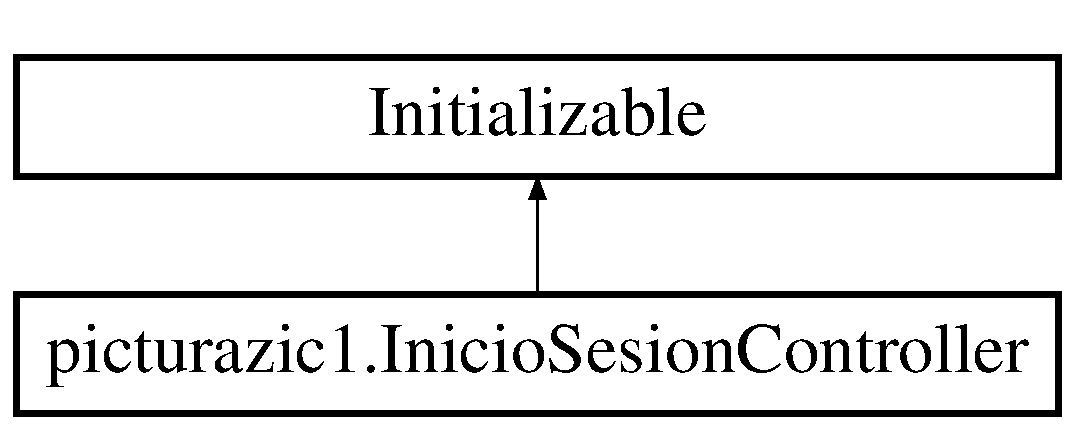
\includegraphics[height=2.000000cm]{classpicturazic1_1_1_inicio_sesion_controller}
\end{center}
\end{figure}
\subsection*{Public Member Functions}
\begin{DoxyCompactItemize}
\item 
void \mbox{\hyperlink{classpicturazic1_1_1_inicio_sesion_controller_a879e972a8f81ff3e4edc41244d371a25}{initialize}} (U\+RL url, Resource\+Bundle rb)
\item 
\mbox{\Hypertarget{classpicturazic1_1_1_inicio_sesion_controller_aeaf1ade35872452a404289bfedf208d1}\label{classpicturazic1_1_1_inicio_sesion_controller_aeaf1ade35872452a404289bfedf208d1}} 
\mbox{\hyperlink{classmodelo_1_1_usuario}{Usuario}} {\bfseries iniciar\+Sesion} ()
\item 
\mbox{\Hypertarget{classpicturazic1_1_1_inicio_sesion_controller_ae443843ad93c8690e2ead2c9c88c13a7}\label{classpicturazic1_1_1_inicio_sesion_controller_ae443843ad93c8690e2ead2c9c88c13a7}} 
void {\bfseries llenar} (String n, String p)
\end{DoxyCompactItemize}


\subsection{Detailed Description}
F\+X\+ML Controller class

\begin{DoxyAuthor}{Author}
HW 
\end{DoxyAuthor}


\subsection{Member Function Documentation}
\mbox{\Hypertarget{classpicturazic1_1_1_inicio_sesion_controller_a879e972a8f81ff3e4edc41244d371a25}\label{classpicturazic1_1_1_inicio_sesion_controller_a879e972a8f81ff3e4edc41244d371a25}} 
\index{picturazic1\+::\+Inicio\+Sesion\+Controller@{picturazic1\+::\+Inicio\+Sesion\+Controller}!initialize@{initialize}}
\index{initialize@{initialize}!picturazic1\+::\+Inicio\+Sesion\+Controller@{picturazic1\+::\+Inicio\+Sesion\+Controller}}
\subsubsection{\texorpdfstring{initialize()}{initialize()}}
{\footnotesize\ttfamily void picturazic1.\+Inicio\+Sesion\+Controller.\+initialize (\begin{DoxyParamCaption}\item[{U\+RL}]{url,  }\item[{Resource\+Bundle}]{rb }\end{DoxyParamCaption})}

Initializes the controller class. 

The documentation for this class was generated from the following file\+:\begin{DoxyCompactItemize}
\item 
D\+:/\+Escritorio/\+Clase/20172018/\+Eclipse Workspace/\+Picturasic/src/picturazic1/Inicio\+Sesion\+Controller.\+java\end{DoxyCompactItemize}

\hypertarget{classpicturazic1_1_1_panel_comentario_controller}{}\section{picturazic1.\+Panel\+Comentario\+Controller Class Reference}
\label{classpicturazic1_1_1_panel_comentario_controller}\index{picturazic1.\+Panel\+Comentario\+Controller@{picturazic1.\+Panel\+Comentario\+Controller}}
Inheritance diagram for picturazic1.\+Panel\+Comentario\+Controller\+:\begin{figure}[H]
\begin{center}
\leavevmode
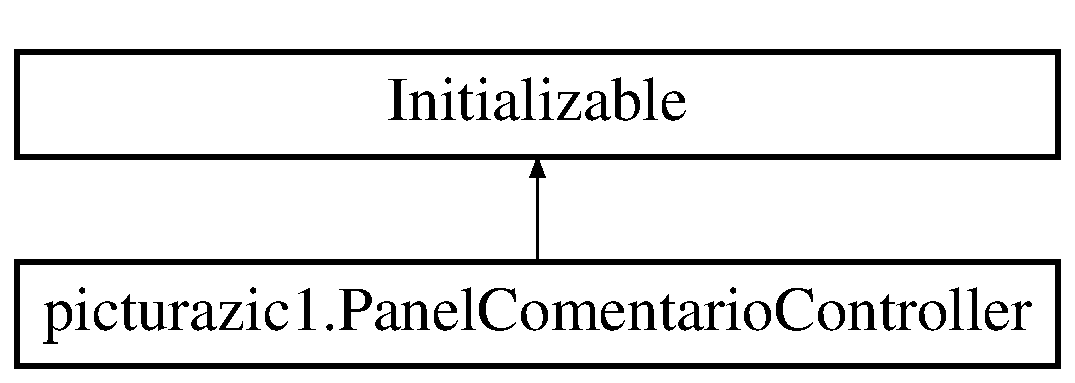
\includegraphics[height=2.000000cm]{classpicturazic1_1_1_panel_comentario_controller}
\end{center}
\end{figure}
\subsection*{Public Member Functions}
\begin{DoxyCompactItemize}
\item 
void \mbox{\hyperlink{classpicturazic1_1_1_panel_comentario_controller_ac68b1c64d3e043f88b67b906230bb55e}{initialize}} (U\+RL url, Resource\+Bundle rb)
\end{DoxyCompactItemize}


\subsection{Detailed Description}
F\+X\+ML Controller class

\begin{DoxyAuthor}{Author}
HW 
\end{DoxyAuthor}


\subsection{Member Function Documentation}
\mbox{\Hypertarget{classpicturazic1_1_1_panel_comentario_controller_ac68b1c64d3e043f88b67b906230bb55e}\label{classpicturazic1_1_1_panel_comentario_controller_ac68b1c64d3e043f88b67b906230bb55e}} 
\index{picturazic1\+::\+Panel\+Comentario\+Controller@{picturazic1\+::\+Panel\+Comentario\+Controller}!initialize@{initialize}}
\index{initialize@{initialize}!picturazic1\+::\+Panel\+Comentario\+Controller@{picturazic1\+::\+Panel\+Comentario\+Controller}}
\subsubsection{\texorpdfstring{initialize()}{initialize()}}
{\footnotesize\ttfamily void picturazic1.\+Panel\+Comentario\+Controller.\+initialize (\begin{DoxyParamCaption}\item[{U\+RL}]{url,  }\item[{Resource\+Bundle}]{rb }\end{DoxyParamCaption})}

Initializes the controller class. 

The documentation for this class was generated from the following file\+:\begin{DoxyCompactItemize}
\item 
D\+:/\+Escritorio/\+Clase/20172018/\+Eclipse Workspace/\+Picturasic/src/picturazic1/Panel\+Comentario\+Controller.\+java\end{DoxyCompactItemize}

\hypertarget{classpicturazic1_1_1_participar_controller}{}\section{picturazic1.\+Participar\+Controller Class Reference}
\label{classpicturazic1_1_1_participar_controller}\index{picturazic1.\+Participar\+Controller@{picturazic1.\+Participar\+Controller}}
Inheritance diagram for picturazic1.\+Participar\+Controller\+:\begin{figure}[H]
\begin{center}
\leavevmode
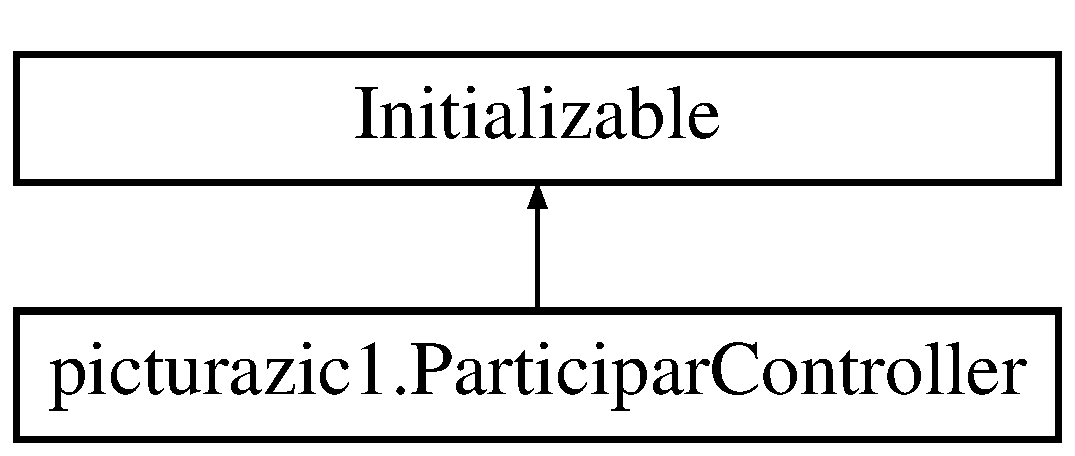
\includegraphics[height=2.000000cm]{classpicturazic1_1_1_participar_controller}
\end{center}
\end{figure}
\subsection*{Public Member Functions}
\begin{DoxyCompactItemize}
\item 
void \mbox{\hyperlink{classpicturazic1_1_1_participar_controller_a73c5f79e43aa45114e7bd176d3839dac}{initialize}} (U\+RL url, Resource\+Bundle rb)
\item 
\mbox{\Hypertarget{classpicturazic1_1_1_participar_controller_aa04fcd549667f6df333e31253a7fa026}\label{classpicturazic1_1_1_participar_controller_aa04fcd549667f6df333e31253a7fa026}} 
void {\bfseries pasar\+Stage} (Stage stage, \mbox{\hyperlink{classmodelo_1_1_usuario}{Usuario}} u)
\item 
\mbox{\Hypertarget{classpicturazic1_1_1_participar_controller_aca507bdc034f9f52c346931a37faec33}\label{classpicturazic1_1_1_participar_controller_aca507bdc034f9f52c346931a37faec33}} 
void {\bfseries inicializar\+Reto} (\mbox{\hyperlink{classmodelo_1_1_reto}{Reto}} reto)
\end{DoxyCompactItemize}


\subsection{Detailed Description}
F\+X\+ML Controller class

\begin{DoxyAuthor}{Author}
HW 
\end{DoxyAuthor}


\subsection{Member Function Documentation}
\mbox{\Hypertarget{classpicturazic1_1_1_participar_controller_a73c5f79e43aa45114e7bd176d3839dac}\label{classpicturazic1_1_1_participar_controller_a73c5f79e43aa45114e7bd176d3839dac}} 
\index{picturazic1\+::\+Participar\+Controller@{picturazic1\+::\+Participar\+Controller}!initialize@{initialize}}
\index{initialize@{initialize}!picturazic1\+::\+Participar\+Controller@{picturazic1\+::\+Participar\+Controller}}
\subsubsection{\texorpdfstring{initialize()}{initialize()}}
{\footnotesize\ttfamily void picturazic1.\+Participar\+Controller.\+initialize (\begin{DoxyParamCaption}\item[{U\+RL}]{url,  }\item[{Resource\+Bundle}]{rb }\end{DoxyParamCaption})}

Initializes the controller class. 

The documentation for this class was generated from the following file\+:\begin{DoxyCompactItemize}
\item 
D\+:/\+Escritorio/\+Clase/20172018/\+Eclipse Workspace/\+Picturasic/src/picturazic1/Participar\+Controller.\+java\end{DoxyCompactItemize}

\hypertarget{classpicturazic1_1_1_perfil_controller}{}\section{picturazic1.\+Perfil\+Controller Class Reference}
\label{classpicturazic1_1_1_perfil_controller}\index{picturazic1.\+Perfil\+Controller@{picturazic1.\+Perfil\+Controller}}
Inheritance diagram for picturazic1.\+Perfil\+Controller\+:\begin{figure}[H]
\begin{center}
\leavevmode
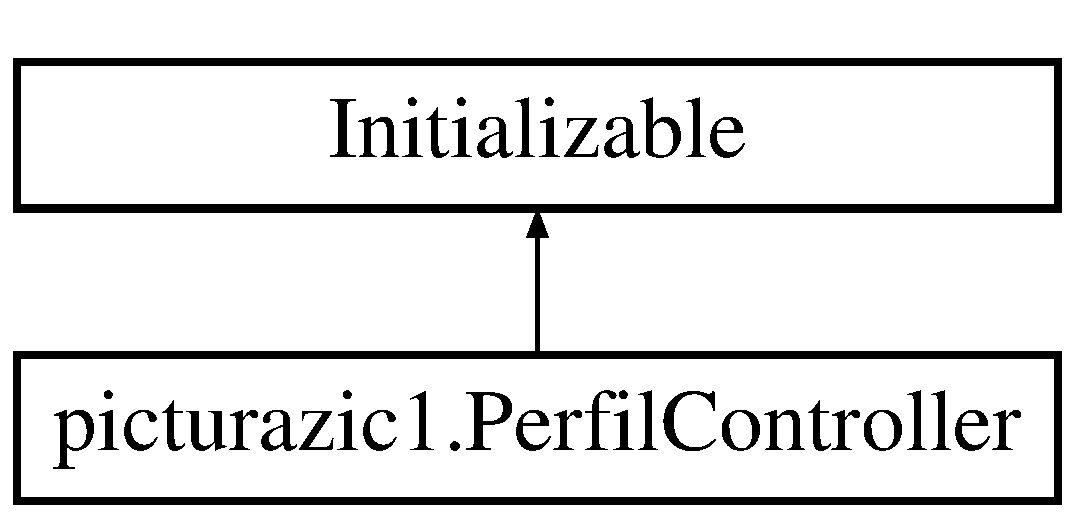
\includegraphics[height=2.000000cm]{classpicturazic1_1_1_perfil_controller}
\end{center}
\end{figure}
\subsection*{Public Member Functions}
\begin{DoxyCompactItemize}
\item 
void \mbox{\hyperlink{classpicturazic1_1_1_perfil_controller_afd50104608ebc66473ab172ccad35a3f}{initialize}} (U\+RL url, Resource\+Bundle rb)
\item 
\mbox{\Hypertarget{classpicturazic1_1_1_perfil_controller_a8303f3c409821b211ad8f31b9a24741a}\label{classpicturazic1_1_1_perfil_controller_a8303f3c409821b211ad8f31b9a24741a}} 
void {\bfseries obtener\+Usuario} (\mbox{\hyperlink{classmodelo_1_1_usuario}{Usuario}} u)
\item 
\mbox{\Hypertarget{classpicturazic1_1_1_perfil_controller_a1bc99be85b12824079e7a1a9d24cbffe}\label{classpicturazic1_1_1_perfil_controller_a1bc99be85b12824079e7a1a9d24cbffe}} 
void {\bfseries cargar\+Usuario} (\mbox{\hyperlink{classmodelo_1_1_usuario}{Usuario}} usuario)
\item 
\mbox{\Hypertarget{classpicturazic1_1_1_perfil_controller_a57efaadc2a0b6ce69ebc2a5ef2220f1c}\label{classpicturazic1_1_1_perfil_controller_a57efaadc2a0b6ce69ebc2a5ef2220f1c}} 
List$<$ \mbox{\hyperlink{classmodelo_1_1_usuario}{Usuario}} $>$ {\bfseries obtener\+Usuarios} ()
\end{DoxyCompactItemize}


\subsection{Detailed Description}
F\+X\+ML Controller class

\begin{DoxyAuthor}{Author}
HW 
\end{DoxyAuthor}


\subsection{Member Function Documentation}
\mbox{\Hypertarget{classpicturazic1_1_1_perfil_controller_afd50104608ebc66473ab172ccad35a3f}\label{classpicturazic1_1_1_perfil_controller_afd50104608ebc66473ab172ccad35a3f}} 
\index{picturazic1\+::\+Perfil\+Controller@{picturazic1\+::\+Perfil\+Controller}!initialize@{initialize}}
\index{initialize@{initialize}!picturazic1\+::\+Perfil\+Controller@{picturazic1\+::\+Perfil\+Controller}}
\subsubsection{\texorpdfstring{initialize()}{initialize()}}
{\footnotesize\ttfamily void picturazic1.\+Perfil\+Controller.\+initialize (\begin{DoxyParamCaption}\item[{U\+RL}]{url,  }\item[{Resource\+Bundle}]{rb }\end{DoxyParamCaption})}

Initializes the controller class. 

The documentation for this class was generated from the following file\+:\begin{DoxyCompactItemize}
\item 
D\+:/\+Escritorio/\+Clase/20172018/\+Eclipse Workspace/\+Picturasic/src/picturazic1/Perfil\+Controller.\+java\end{DoxyCompactItemize}

\hypertarget{classpicturazic1_1_1_picturazic10}{}\section{picturazic1.\+Picturazic10 Class Reference}
\label{classpicturazic1_1_1_picturazic10}\index{picturazic1.\+Picturazic10@{picturazic1.\+Picturazic10}}
Inheritance diagram for picturazic1.\+Picturazic10\+:\begin{figure}[H]
\begin{center}
\leavevmode
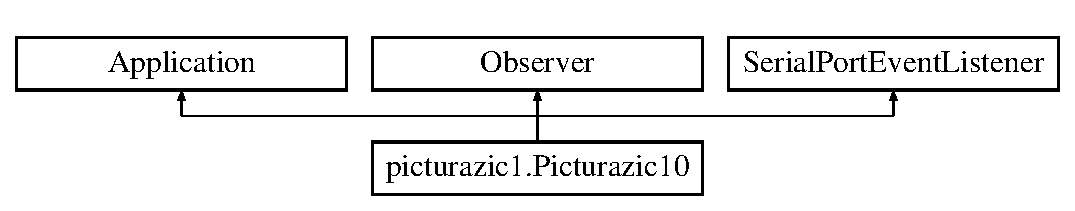
\includegraphics[height=2.000000cm]{classpicturazic1_1_1_picturazic10}
\end{center}
\end{figure}
\subsection*{Public Member Functions}
\begin{DoxyCompactItemize}
\item 
\mbox{\Hypertarget{classpicturazic1_1_1_picturazic10_a2731c2a778924eb66bde5406f5f3ef26}\label{classpicturazic1_1_1_picturazic10_a2731c2a778924eb66bde5406f5f3ef26}} 
void {\bfseries start} (Stage stage)  throws Exception 
\item 
\mbox{\Hypertarget{classpicturazic1_1_1_picturazic10_ab3685d4191fbbe385020ba3d294a15ea}\label{classpicturazic1_1_1_picturazic10_ab3685d4191fbbe385020ba3d294a15ea}} 
void {\bfseries apagar} ()  throws Serial\+Port\+Exception 
\item 
\mbox{\Hypertarget{classpicturazic1_1_1_picturazic10_a53213b757dbc043a8b1be5ad80f1bdd2}\label{classpicturazic1_1_1_picturazic10_a53213b757dbc043a8b1be5ad80f1bdd2}} 
void {\bfseries ventana\+Principal} (Stage stage)  throws I\+O\+Exception 
\item 
\mbox{\Hypertarget{classpicturazic1_1_1_picturazic10_abe51d65faf87c4ff80d4b0bf511c308a}\label{classpicturazic1_1_1_picturazic10_abe51d65faf87c4ff80d4b0bf511c308a}} 
void {\bfseries ventana\+Login} (Stage stage)  throws I\+O\+Exception 
\item 
\mbox{\Hypertarget{classpicturazic1_1_1_picturazic10_a252ea1187b88f79dec0836044f272ee7}\label{classpicturazic1_1_1_picturazic10_a252ea1187b88f79dec0836044f272ee7}} 
void {\bfseries asignar\+Funciones\+Login} ()
\item 
\mbox{\Hypertarget{classpicturazic1_1_1_picturazic10_acd9f0adcdd39732fa91d122fba7c2928}\label{classpicturazic1_1_1_picturazic10_acd9f0adcdd39732fa91d122fba7c2928}} 
void {\bfseries asignar\+Funciones} ()
\item 
\mbox{\Hypertarget{classpicturazic1_1_1_picturazic10_a23b5d40188f5e3c998e64289e5fbd924}\label{classpicturazic1_1_1_picturazic10_a23b5d40188f5e3c998e64289e5fbd924}} 
void {\bfseries mostrar\+Retos} ()  throws I\+O\+Exception 
\item 
\mbox{\Hypertarget{classpicturazic1_1_1_picturazic10_a9286e76ca28baaa48f1ed4631b9ba40a}\label{classpicturazic1_1_1_picturazic10_a9286e76ca28baaa48f1ed4631b9ba40a}} 
void {\bfseries logearse} (String usuario, String contrase�a)  throws I\+O\+Exception 
\item 
\mbox{\Hypertarget{classpicturazic1_1_1_picturazic10_ad82e6b1ebbf51c03f4db46fc5b8b2cbc}\label{classpicturazic1_1_1_picturazic10_ad82e6b1ebbf51c03f4db46fc5b8b2cbc}} 
void {\bfseries singearse} ()
\item 
\mbox{\Hypertarget{classpicturazic1_1_1_picturazic10_aecc1e6ee83bed40313f7d6ede67ae1e8}\label{classpicturazic1_1_1_picturazic10_aecc1e6ee83bed40313f7d6ede67ae1e8}} 
void {\bfseries update} (Observable o, Object arg)
\item 
void \mbox{\hyperlink{classpicturazic1_1_1_picturazic10_a2370148493c564db534dcc32f7bdec90}{serial\+Event}} (Serial\+Port\+Event event)
\item 
\mbox{\Hypertarget{classpicturazic1_1_1_picturazic10_a458ec2978fcc4efa64cc4b772bf61f08}\label{classpicturazic1_1_1_picturazic10_a458ec2978fcc4efa64cc4b772bf61f08}} 
void {\bfseries escribir} (String texto)
\end{DoxyCompactItemize}
\subsection*{Static Public Member Functions}
\begin{DoxyCompactItemize}
\item 
static void \mbox{\hyperlink{classpicturazic1_1_1_picturazic10_a60125dfe777e02320c4ede1ab7901415}{main}} (String\mbox{[}$\,$\mbox{]} args)
\end{DoxyCompactItemize}


\subsection{Detailed Description}
\begin{DoxyAuthor}{Author}
HW 
\end{DoxyAuthor}


\subsection{Member Function Documentation}
\mbox{\Hypertarget{classpicturazic1_1_1_picturazic10_a60125dfe777e02320c4ede1ab7901415}\label{classpicturazic1_1_1_picturazic10_a60125dfe777e02320c4ede1ab7901415}} 
\index{picturazic1\+::\+Picturazic10@{picturazic1\+::\+Picturazic10}!main@{main}}
\index{main@{main}!picturazic1\+::\+Picturazic10@{picturazic1\+::\+Picturazic10}}
\subsubsection{\texorpdfstring{main()}{main()}}
{\footnotesize\ttfamily static void picturazic1.\+Picturazic10.\+main (\begin{DoxyParamCaption}\item[{String \mbox{[}$\,$\mbox{]}}]{args }\end{DoxyParamCaption})\hspace{0.3cm}{\ttfamily [static]}}


\begin{DoxyParams}{Parameters}
{\em args} & the command line arguments \\
\hline
\end{DoxyParams}
\mbox{\Hypertarget{classpicturazic1_1_1_picturazic10_a2370148493c564db534dcc32f7bdec90}\label{classpicturazic1_1_1_picturazic10_a2370148493c564db534dcc32f7bdec90}} 
\index{picturazic1\+::\+Picturazic10@{picturazic1\+::\+Picturazic10}!serial\+Event@{serial\+Event}}
\index{serial\+Event@{serial\+Event}!picturazic1\+::\+Picturazic10@{picturazic1\+::\+Picturazic10}}
\subsubsection{\texorpdfstring{serial\+Event()}{serialEvent()}}
{\footnotesize\ttfamily void picturazic1.\+Picturazic10.\+serial\+Event (\begin{DoxyParamCaption}\item[{Serial\+Port\+Event}]{event }\end{DoxyParamCaption})}

If D\+SR line has changed state 

The documentation for this class was generated from the following file\+:\begin{DoxyCompactItemize}
\item 
D\+:/\+Escritorio/\+Clase/20172018/\+Eclipse Workspace/\+Picturasic/src/picturazic1/Picturazic10.\+java\end{DoxyCompactItemize}

\hypertarget{classmodelo_1_1_reto}{}\section{modelo.\+Reto Class Reference}
\label{classmodelo_1_1_reto}\index{modelo.\+Reto@{modelo.\+Reto}}
Inheritance diagram for modelo.\+Reto\+:\begin{figure}[H]
\begin{center}
\leavevmode
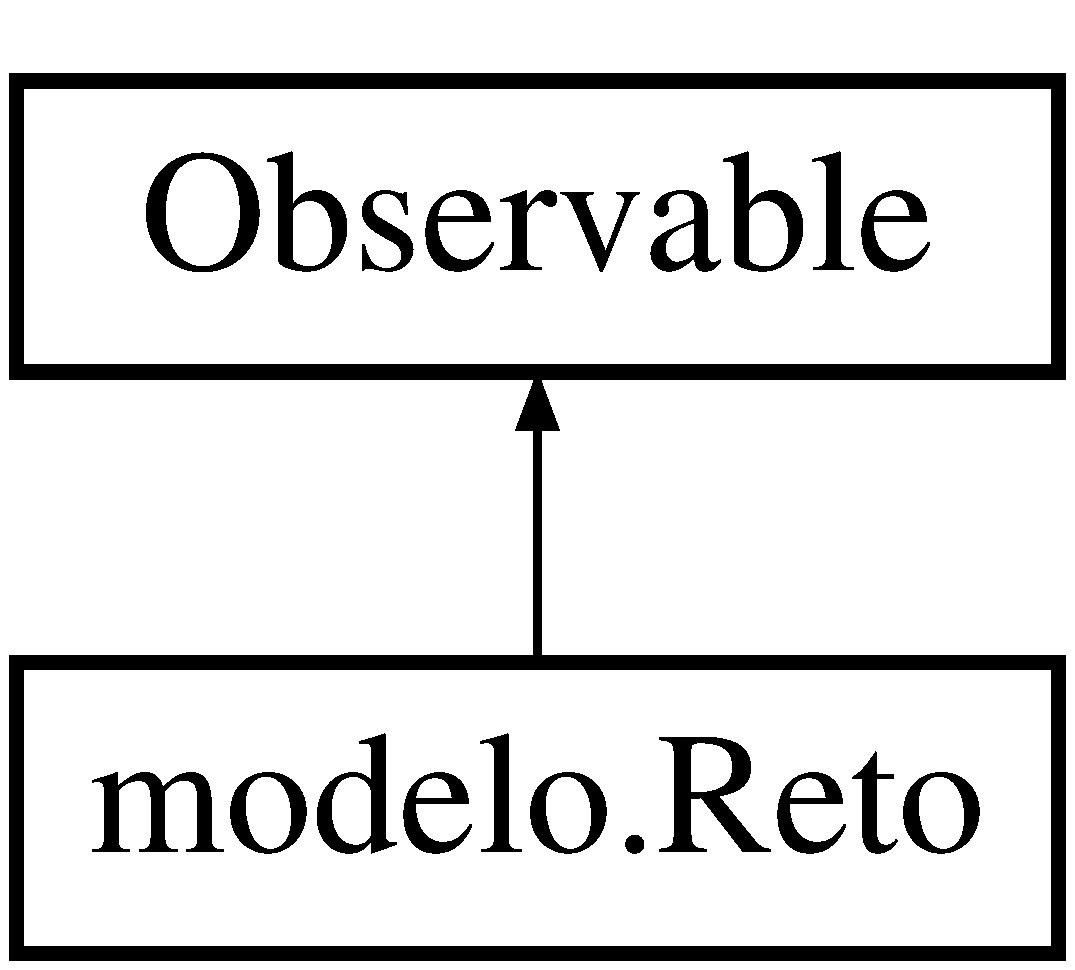
\includegraphics[height=2.000000cm]{classmodelo_1_1_reto}
\end{center}
\end{figure}
\subsection*{Public Member Functions}
\begin{DoxyCompactItemize}
\item 
\mbox{\Hypertarget{classmodelo_1_1_reto_a74b04056a33a865552a5dae69527e5af}\label{classmodelo_1_1_reto_a74b04056a33a865552a5dae69527e5af}} 
{\bfseries Reto} (int reto\+Id, String descripcion, Buffered\+Image ejemplo, String fecha, String titulo)
\item 
\mbox{\Hypertarget{classmodelo_1_1_reto_adb1538f92e9e9b91269c036bad2f6695}\label{classmodelo_1_1_reto_adb1538f92e9e9b91269c036bad2f6695}} 
String {\bfseries get\+Titulo} ()
\item 
\mbox{\Hypertarget{classmodelo_1_1_reto_a86c6df368bfd3ab8c874aa35cb05f31e}\label{classmodelo_1_1_reto_a86c6df368bfd3ab8c874aa35cb05f31e}} 
void {\bfseries participar\+Reto} ()
\item 
\mbox{\Hypertarget{classmodelo_1_1_reto_afc1df072ba256ef71a8f24b8948ffd0c}\label{classmodelo_1_1_reto_afc1df072ba256ef71a8f24b8948ffd0c}} 
void {\bfseries cancelar\+Reto} ()
\item 
\mbox{\Hypertarget{classmodelo_1_1_reto_a3ce96e348237630218cb51d36001c3dc}\label{classmodelo_1_1_reto_a3ce96e348237630218cb51d36001c3dc}} 
\mbox{\hyperlink{classmodelo_1_1_reto}{Reto}} {\bfseries cogeme} ()
\item 
\mbox{\Hypertarget{classmodelo_1_1_reto_ac553f503faff59b1a41934052f60f2bb}\label{classmodelo_1_1_reto_ac553f503faff59b1a41934052f60f2bb}} 
void {\bfseries subir\+Imagen} (String decripcion, String imagen, int usuario, String fecha)
\item 
\mbox{\Hypertarget{classmodelo_1_1_reto_a4dc82f077a5a7442ab6429f88dfb8257}\label{classmodelo_1_1_reto_a4dc82f077a5a7442ab6429f88dfb8257}} 
int {\bfseries get\+Reto\+Id} ()
\item 
\mbox{\Hypertarget{classmodelo_1_1_reto_a8d693de1123ad17b8cc1d4ea7b3516d9}\label{classmodelo_1_1_reto_a8d693de1123ad17b8cc1d4ea7b3516d9}} 
String {\bfseries get\+Descripcion} ()
\item 
\mbox{\Hypertarget{classmodelo_1_1_reto_a41fa7849d955aa7291479fabbffe841e}\label{classmodelo_1_1_reto_a41fa7849d955aa7291479fabbffe841e}} 
Buffered\+Image {\bfseries get\+Ejemplo} ()
\item 
\mbox{\Hypertarget{classmodelo_1_1_reto_a1c972ef5b1c0c6b22b923394a091fb06}\label{classmodelo_1_1_reto_a1c972ef5b1c0c6b22b923394a091fb06}} 
String {\bfseries get\+Fecha} ()
\end{DoxyCompactItemize}
\subsection*{Static Public Member Functions}
\begin{DoxyCompactItemize}
\item 
\mbox{\Hypertarget{classmodelo_1_1_reto_a24ad1371910508220819a560e55687ec}\label{classmodelo_1_1_reto_a24ad1371910508220819a560e55687ec}} 
static \mbox{\hyperlink{classmodelo_1_1_reto}{Reto}} {\bfseries obtener\+Reto\+Por\+Id} (int reto\+Id)
\item 
\mbox{\Hypertarget{classmodelo_1_1_reto_a306160df168610c8b158853d312f37b3}\label{classmodelo_1_1_reto_a306160df168610c8b158853d312f37b3}} 
static List$<$ \mbox{\hyperlink{classmodelo_1_1_reto}{Reto}} $>$ {\bfseries obtener\+Retos\+Diarios} (int id\+User)
\end{DoxyCompactItemize}


\subsection{Detailed Description}
\begin{DoxyAuthor}{Author}
HW 
\end{DoxyAuthor}


The documentation for this class was generated from the following file\+:\begin{DoxyCompactItemize}
\item 
D\+:/\+Escritorio/\+Clase/20172018/\+Eclipse Workspace/\+Picturasic/src/modelo/Reto.\+java\end{DoxyCompactItemize}

\hypertarget{classpicturazic1_1_1_reto_controller}{}\section{picturazic1.\+Reto\+Controller Class Reference}
\label{classpicturazic1_1_1_reto_controller}\index{picturazic1.\+Reto\+Controller@{picturazic1.\+Reto\+Controller}}
Inheritance diagram for picturazic1.\+Reto\+Controller\+:\begin{figure}[H]
\begin{center}
\leavevmode
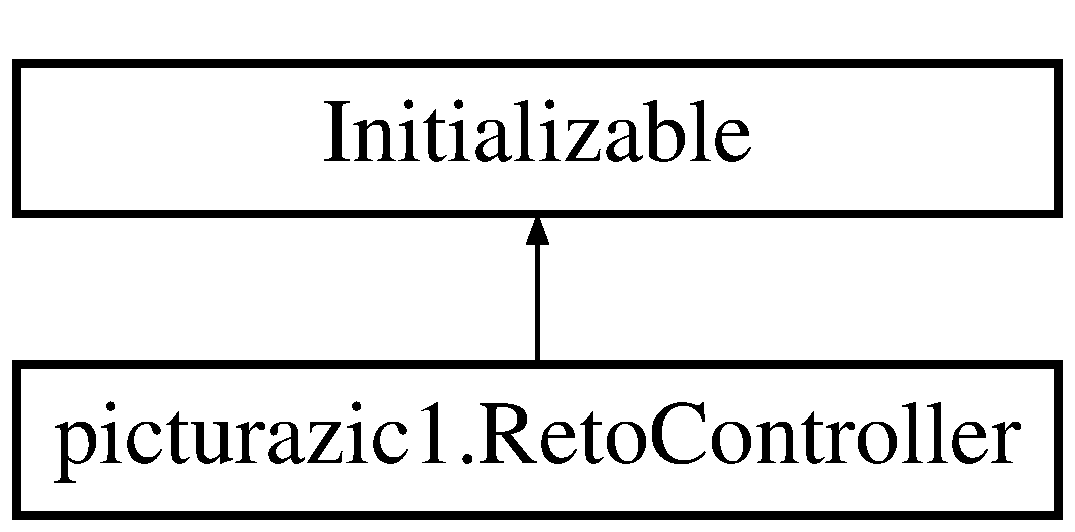
\includegraphics[height=2.000000cm]{classpicturazic1_1_1_reto_controller}
\end{center}
\end{figure}
\subsection*{Public Member Functions}
\begin{DoxyCompactItemize}
\item 
void \mbox{\hyperlink{classpicturazic1_1_1_reto_controller_a48a8cd99d528c1712df7a7c3a8ce20b2}{initialize}} (U\+RL url, Resource\+Bundle rb)
\item 
\mbox{\Hypertarget{classpicturazic1_1_1_reto_controller_a6b487b3de21e49fde92a8330cb304632}\label{classpicturazic1_1_1_reto_controller_a6b487b3de21e49fde92a8330cb304632}} 
void {\bfseries crear\+Reto} (\mbox{\hyperlink{classmodelo_1_1_reto}{Reto}} reto)
\end{DoxyCompactItemize}


\subsection{Detailed Description}
F\+X\+ML Controller class

\begin{DoxyAuthor}{Author}
HW 
\end{DoxyAuthor}


\subsection{Member Function Documentation}
\mbox{\Hypertarget{classpicturazic1_1_1_reto_controller_a48a8cd99d528c1712df7a7c3a8ce20b2}\label{classpicturazic1_1_1_reto_controller_a48a8cd99d528c1712df7a7c3a8ce20b2}} 
\index{picturazic1\+::\+Reto\+Controller@{picturazic1\+::\+Reto\+Controller}!initialize@{initialize}}
\index{initialize@{initialize}!picturazic1\+::\+Reto\+Controller@{picturazic1\+::\+Reto\+Controller}}
\subsubsection{\texorpdfstring{initialize()}{initialize()}}
{\footnotesize\ttfamily void picturazic1.\+Reto\+Controller.\+initialize (\begin{DoxyParamCaption}\item[{U\+RL}]{url,  }\item[{Resource\+Bundle}]{rb }\end{DoxyParamCaption})}

Initializes the controller class. 

The documentation for this class was generated from the following file\+:\begin{DoxyCompactItemize}
\item 
D\+:/\+Escritorio/\+Clase/20172018/\+Eclipse Workspace/\+Picturasic/src/picturazic1/Reto\+Controller.\+java\end{DoxyCompactItemize}

\hypertarget{classpicturazic1_1_1_send_attachment_in_email}{}\section{picturazic1.\+Send\+Attachment\+In\+Email Class Reference}
\label{classpicturazic1_1_1_send_attachment_in_email}\index{picturazic1.\+Send\+Attachment\+In\+Email@{picturazic1.\+Send\+Attachment\+In\+Email}}
\subsection*{Static Public Member Functions}
\begin{DoxyCompactItemize}
\item 
\mbox{\Hypertarget{classpicturazic1_1_1_send_attachment_in_email_a4824d1920e4e1685ed102a499d393faa}\label{classpicturazic1_1_1_send_attachment_in_email_a4824d1920e4e1685ed102a499d393faa}} 
static void {\bfseries mail} (String filepath, String email\+Dest)
\end{DoxyCompactItemize}


The documentation for this class was generated from the following file\+:\begin{DoxyCompactItemize}
\item 
D\+:/\+Escritorio/\+Clase/20172018/\+Eclipse Workspace/\+Picturasic/src/picturazic1/Send\+Attachment\+In\+Email.\+java\end{DoxyCompactItemize}

\hypertarget{classpicturazic1_1_1_serial_listener}{}\section{picturazic1.\+Serial\+Listener Class Reference}
\label{classpicturazic1_1_1_serial_listener}\index{picturazic1.\+Serial\+Listener@{picturazic1.\+Serial\+Listener}}
Inheritance diagram for picturazic1.\+Serial\+Listener\+:\begin{figure}[H]
\begin{center}
\leavevmode
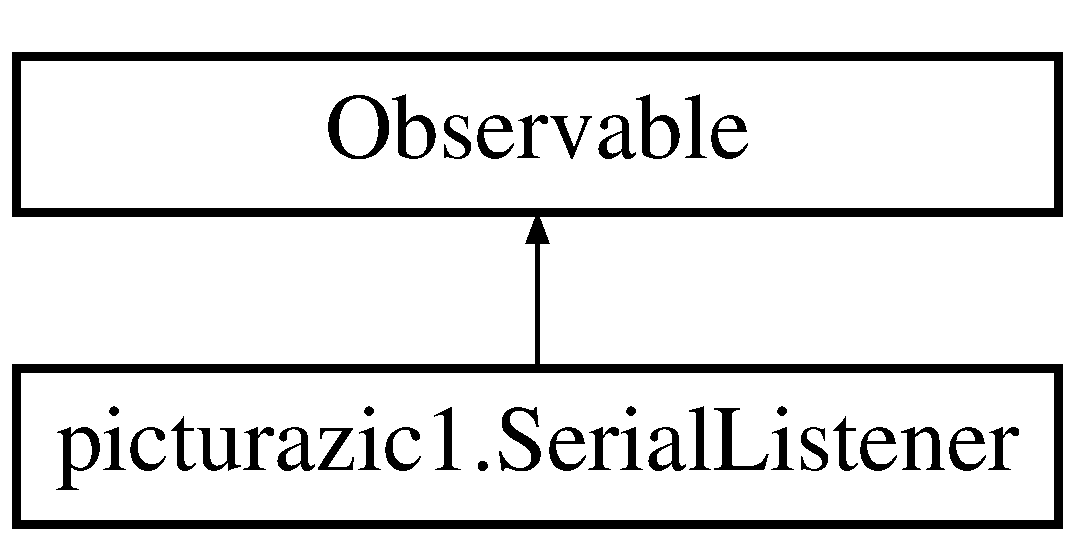
\includegraphics[height=2.000000cm]{classpicturazic1_1_1_serial_listener}
\end{center}
\end{figure}
\subsection*{Classes}
\begin{DoxyCompactItemize}
\item 
class {\bfseries Serial\+Port\+Reader}
\end{DoxyCompactItemize}
\subsection*{Public Member Functions}
\begin{DoxyCompactItemize}
\item 
\mbox{\Hypertarget{classpicturazic1_1_1_serial_listener_a30ddb0a9805bb37a5e63f4bbbec3a3a3}\label{classpicturazic1_1_1_serial_listener_a30ddb0a9805bb37a5e63f4bbbec3a3a3}} 
{\bfseries Serial\+Listener} (\mbox{\hyperlink{classpicturazic1_1_1_picturazic10}{Picturazic10}} a)  throws Serial\+Port\+Exception 
\item 
\mbox{\Hypertarget{classpicturazic1_1_1_serial_listener_a28d7e5c2656d6af44622d91c3423915b}\label{classpicturazic1_1_1_serial_listener_a28d7e5c2656d6af44622d91c3423915b}} 
void {\bfseries add\+Lis} ()  throws Serial\+Port\+Exception 
\end{DoxyCompactItemize}
\subsection*{Static Public Member Functions}
\begin{DoxyCompactItemize}
\item 
\mbox{\Hypertarget{classpicturazic1_1_1_serial_listener_a2683a715f60b1c01938fdfc04b98d236}\label{classpicturazic1_1_1_serial_listener_a2683a715f60b1c01938fdfc04b98d236}} 
static void {\bfseries leido} (String texto\+Leido)
\item 
\mbox{\Hypertarget{classpicturazic1_1_1_serial_listener_a6066df8dee153fc3e406f5951610a954}\label{classpicturazic1_1_1_serial_listener_a6066df8dee153fc3e406f5951610a954}} 
static void {\bfseries escribir} (String texto)
\end{DoxyCompactItemize}


The documentation for this class was generated from the following file\+:\begin{DoxyCompactItemize}
\item 
D\+:/\+Escritorio/\+Clase/20172018/\+Eclipse Workspace/\+Picturasic/src/picturazic1/Serial\+Listener.\+java\end{DoxyCompactItemize}

\hypertarget{classmodelo_1_1_usuario}{}\section{modelo.\+Usuario Class Reference}
\label{classmodelo_1_1_usuario}\index{modelo.\+Usuario@{modelo.\+Usuario}}
Inheritance diagram for modelo.\+Usuario\+:\begin{figure}[H]
\begin{center}
\leavevmode
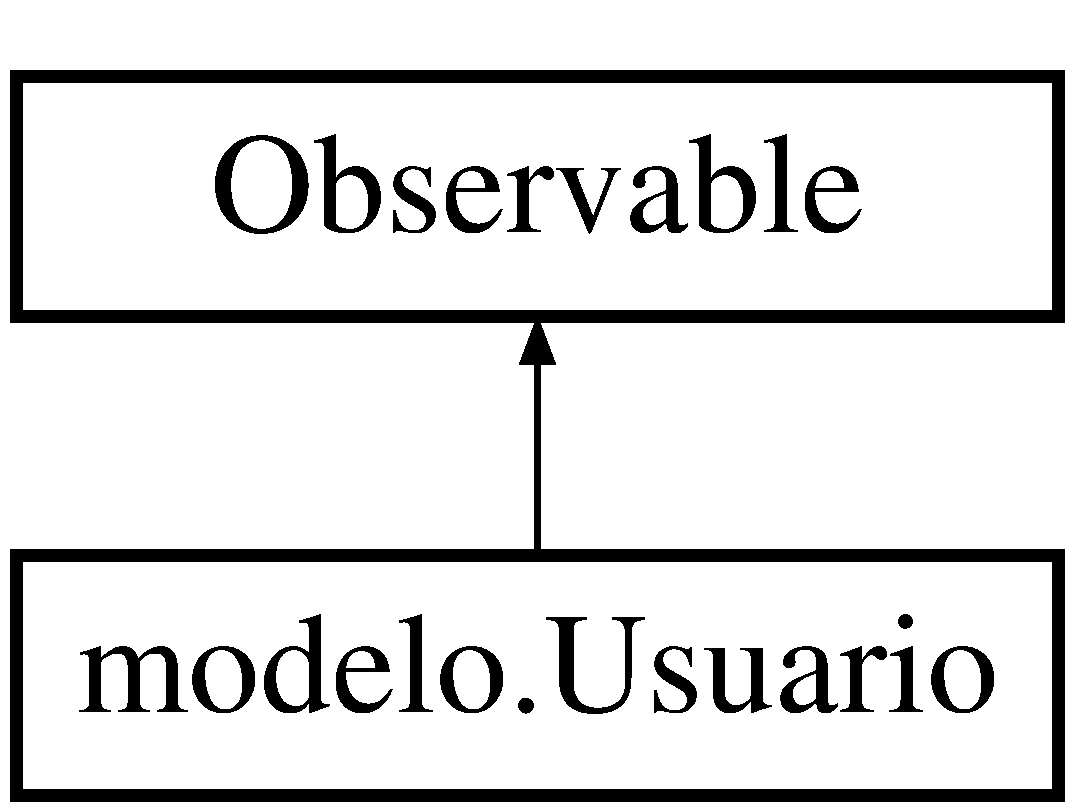
\includegraphics[height=2.000000cm]{classmodelo_1_1_usuario}
\end{center}
\end{figure}
\subsection*{Public Member Functions}
\begin{DoxyCompactItemize}
\item 
\mbox{\Hypertarget{classmodelo_1_1_usuario_a6070de92838a506458ccd85e4ba64256}\label{classmodelo_1_1_usuario_a6070de92838a506458ccd85e4ba64256}} 
{\bfseries Usuario} (int id, String nombre, String apellido, String correo, String fecha, Buffered\+Image avatar, double experiencia, String username)
\item 
\mbox{\Hypertarget{classmodelo_1_1_usuario_afd9614ab19dbc8d9a63339ba48003519}\label{classmodelo_1_1_usuario_afd9614ab19dbc8d9a63339ba48003519}} 
String {\bfseries get\+Username} ()
\item 
\mbox{\Hypertarget{classmodelo_1_1_usuario_a557ba08b1e96354700e86cb2e4a85ebd}\label{classmodelo_1_1_usuario_a557ba08b1e96354700e86cb2e4a85ebd}} 
void {\bfseries obtener\+Reciompensa} (int recompensa)
\item 
\mbox{\Hypertarget{classmodelo_1_1_usuario_a4f39aac4804e1990385f747e0286c085}\label{classmodelo_1_1_usuario_a4f39aac4804e1990385f747e0286c085}} 
List$<$ \mbox{\hyperlink{classmodelo_1_1_usuario}{Usuario}} $>$ {\bfseries ver\+Seguidores} ()
\item 
\mbox{\Hypertarget{classmodelo_1_1_usuario_a207d20ba99d17f964133d0b5ff9dd26d}\label{classmodelo_1_1_usuario_a207d20ba99d17f964133d0b5ff9dd26d}} 
void {\bfseries seguidores} ()
\item 
\mbox{\Hypertarget{classmodelo_1_1_usuario_acb3327a5d6ca0689910aa78823643f13}\label{classmodelo_1_1_usuario_acb3327a5d6ca0689910aa78823643f13}} 
void {\bfseries ver\+Usuario} ()
\item 
\mbox{\Hypertarget{classmodelo_1_1_usuario_a9b718abb70162e2267dac63871339a91}\label{classmodelo_1_1_usuario_a9b718abb70162e2267dac63871339a91}} 
int {\bfseries get\+Id} ()
\item 
\mbox{\Hypertarget{classmodelo_1_1_usuario_ac0420f9e34ab2d3ca5334444ae7d9ee9}\label{classmodelo_1_1_usuario_ac0420f9e34ab2d3ca5334444ae7d9ee9}} 
String {\bfseries get\+Nombre} ()
\item 
\mbox{\Hypertarget{classmodelo_1_1_usuario_a736af6115a71cba37b4a87ae3430994f}\label{classmodelo_1_1_usuario_a736af6115a71cba37b4a87ae3430994f}} 
String {\bfseries get\+Apellido} ()
\item 
\mbox{\Hypertarget{classmodelo_1_1_usuario_a846c5ccf22a065fda68b6e69b02c1124}\label{classmodelo_1_1_usuario_a846c5ccf22a065fda68b6e69b02c1124}} 
String {\bfseries get\+Correo} ()
\item 
\mbox{\Hypertarget{classmodelo_1_1_usuario_a53b65f7ac848e7bb2c95e55afc019a8b}\label{classmodelo_1_1_usuario_a53b65f7ac848e7bb2c95e55afc019a8b}} 
String {\bfseries get\+Fecha} ()
\item 
\mbox{\Hypertarget{classmodelo_1_1_usuario_a914cdcd3dde8caf9dc05dbdad149d442}\label{classmodelo_1_1_usuario_a914cdcd3dde8caf9dc05dbdad149d442}} 
Buffered\+Image {\bfseries get\+Avatar} ()
\item 
\mbox{\Hypertarget{classmodelo_1_1_usuario_a2e22270ab079a28f765c652d46620fdd}\label{classmodelo_1_1_usuario_a2e22270ab079a28f765c652d46620fdd}} 
double {\bfseries get\+Experiencia} ()
\item 
\mbox{\Hypertarget{classmodelo_1_1_usuario_a74dd866bd4b30e971af4488672eff042}\label{classmodelo_1_1_usuario_a74dd866bd4b30e971af4488672eff042}} 
int {\bfseries get\+Nivel} ()
\item 
\mbox{\Hypertarget{classmodelo_1_1_usuario_af26b4b82bc86a2a3d41fdd722da0a2c3}\label{classmodelo_1_1_usuario_af26b4b82bc86a2a3d41fdd722da0a2c3}} 
double {\bfseries get\+Experiencia\+Nivel\+Actual} ()
\end{DoxyCompactItemize}
\subsection*{Static Public Member Functions}
\begin{DoxyCompactItemize}
\item 
\mbox{\Hypertarget{classmodelo_1_1_usuario_a613c5b0151db527d6fe2366734e6771e}\label{classmodelo_1_1_usuario_a613c5b0151db527d6fe2366734e6771e}} 
static \mbox{\hyperlink{classmodelo_1_1_usuario}{Usuario}} {\bfseries autentificarse} (String user, String passw)
\item 
\mbox{\Hypertarget{classmodelo_1_1_usuario_afe6b558d3e9170ce7948098ab68de905}\label{classmodelo_1_1_usuario_afe6b558d3e9170ce7948098ab68de905}} 
static void {\bfseries crear\+Usuario} (String username, String nombre, String apellido, String correo, String pass)
\item 
\mbox{\Hypertarget{classmodelo_1_1_usuario_a0ec21010c2d3c4bc3061cb9d879ccaf8}\label{classmodelo_1_1_usuario_a0ec21010c2d3c4bc3061cb9d879ccaf8}} 
static void {\bfseries seguir} (int seguidor, int segido)  throws S\+Q\+L\+Exception 
\item 
\mbox{\Hypertarget{classmodelo_1_1_usuario_a19af904ce3274c36fe7dc32a5a9e924c}\label{classmodelo_1_1_usuario_a19af904ce3274c36fe7dc32a5a9e924c}} 
static void {\bfseries verificar\+Usuario} (String \mbox{[}$\,$\mbox{]} datos)
\item 
\mbox{\Hypertarget{classmodelo_1_1_usuario_a106897c3e42a861c5c90664c7907df9f}\label{classmodelo_1_1_usuario_a106897c3e42a861c5c90664c7907df9f}} 
static \mbox{\hyperlink{classmodelo_1_1_usuario}{Usuario}} {\bfseries obtener\+Usuario\+Id} (int id)
\item 
\mbox{\Hypertarget{classmodelo_1_1_usuario_a4d1eaceea4954ca89fd870cd894c230c}\label{classmodelo_1_1_usuario_a4d1eaceea4954ca89fd870cd894c230c}} 
static List$<$ \mbox{\hyperlink{classmodelo_1_1_usuario}{Usuario}} $>$ {\bfseries obtener\+Usuarios} (String username)
\end{DoxyCompactItemize}


\subsection{Detailed Description}
\begin{DoxyAuthor}{Author}
HW 
\end{DoxyAuthor}


The documentation for this class was generated from the following file\+:\begin{DoxyCompactItemize}
\item 
D\+:/\+Escritorio/\+Clase/20172018/\+Eclipse Workspace/\+Picturasic/src/modelo/Usuario.\+java\end{DoxyCompactItemize}

%--- End generated contents ---

% Index
\backmatter
\newpage
\phantomsection
\clearemptydoublepage
\addcontentsline{toc}{chapter}{Index}
\printindex

\end{document}
